\documentclass[tikz,border=4pt]{standalone}
\usepackage{ctex}\usepackage{amsmath}
\usetikzlibrary{arrows.meta,positioning}
\begin{document}
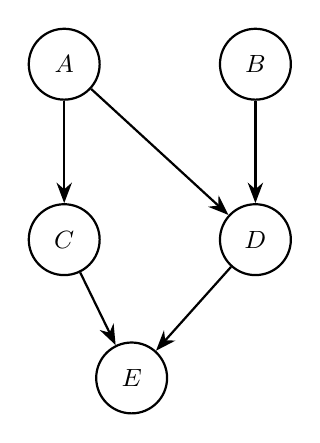
\begin{tikzpicture}[>={Stealth[length=2.6mm]},node distance=1.3cm and 1.5cm,every node/.style={circle,draw,thick,minimum size=9mm,font=\small}]
\node (A) {$A$};
\node (B) [right=of A] {$B$};
\node (C) [below=of A] {$C$};
\node (D) [below=of B] {$D$};
\node (E) [below right=1.1cm and 0.2cm of C] {$E$};
\draw[->,thick] (A)--(C);
\draw[->,thick] (A)--(D);
\draw[->,thick] (B)--(D);
\draw[->,thick] (C)--(E);
\draw[->,thick] (D)--(E);
\end{tikzpicture}
\end{document}
